\section{Scale-up Server Scalalbility}

%$$$$$$$$$$$$$$$$$$$$$$$$$$$$$$$$$$$$$$$$$$$$$$$$$$$$$$$$$$$$$$$$$$$$$$$$$$$$$$$$
%$$$$$$$$$$$$$$$$$$$$$$$$$$$$$$$$$$$$$$$$$$$$$$$$$$$$$$$$$$$$$$$$$$$$$$$$$$$$$$$$
% Apache Spark에 대한 설명
%$$$$$$$$$$$$$$$$$$$$$$$$$$$$$$$$$$$$$$$$$$$$$$$$$$$$$$$$$$$$$$$$$$$$$$$$$$$$$$$$

\ifkor
이번 장에서는 스파크의 Scalalbility에 대해서 설명한다.
\else

\fi

%$$$$$$$$$$$$$$$$$$$$$$$$$$$$$$$$$$$$$$$$$$$$$$$$$$$$$$$$$$$$$$$$$$$$$$$$$$$$$$$$
%$$$$$$$$$$$$$$$$$$$$$$$$$$$$$$$$$$$$$$$$$$$$$$$$$$$$$$$$$$$$$$$$$$$$$$$$$$$$$$$$
% 이번 장에 대한 설명
%$$$$$$$$$$$$$$$$$$$$$$$$$$$$$$$$$$$$$$$$$$$$$$$$$$$$$$$$$$$$$$$$$$$$$$$$$$$$$$$$
\ifkor
벤치마크는 BigData Benchmark를 사용하였다.
\else

\fi

\subsection{Test-Bed and Benchmark}

%$$$$$$$$$$$$$$$$$$$$$$$$$$$$$$$$$$$$$$$$$$$$$$$$$$$$$$$$$$$$$$$$$$$$$$$$$$$$$$$$
%$$$$$$$$$$$$$$$$$$$$$$$$$$$$$$$$$$$$$$$$$$$$$$$$$$$$$$$$$$$$$$$$$$$$$$$$$$$$$$$$
% 테스트 베드 설명
%$$$$$$$$$$$$$$$$$$$$$$$$$$$$$$$$$$$$$$$$$$$$$$$$$$$$$$$$$$$$$$$$$$$$$$$$$$$$$$$$
\ifkor
IBM server에 대한 설명 
\else

\fi


%$$$$$$$$$$$$$$$$$$$$$$$$$$$$$$$$$$$$$$$$$$$$$$$$$$$$$$$$$$$$$$$$$$$$$$$$$$$$$$$$
%$$$$$$$$$$$$$$$$$$$$$$$$$$$$$$$$$$$$$$$$$$$$$$$$$$$$$$$$$$$$$$$$$$$$$$$$$$$$$$$$
%Benchamrk에 대한 설명
%$$$$$$$$$$$$$$$$$$$$$$$$$$$$$$$$$$$$$$$$$$$$$$$$$$$$$$$$$$$$$$$$$$$$$$$$$$$$$$$$
\ifkor
벤치마크와 워크로드에 대한 BigData Benchmark를 사용하였다.
\else

\fi

\subsection{Spark Scalability Problem}


\begin{figure*}[tb]
    \centering
    \begin{subfigure}[b]{0.33\textwidth}
        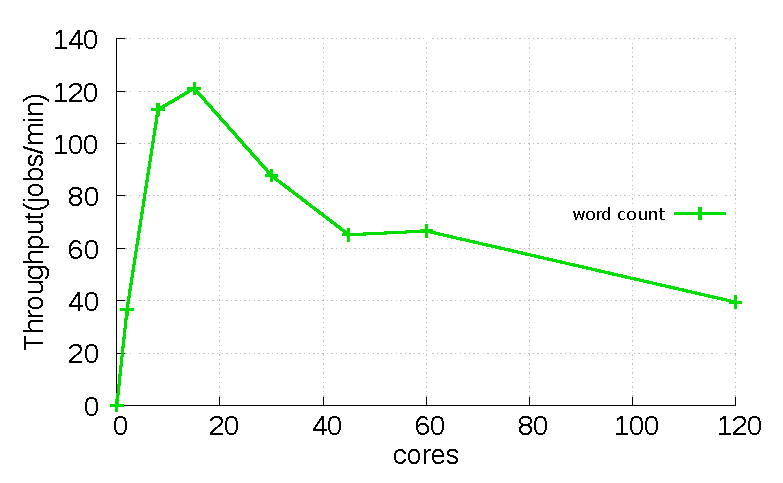
\includegraphics[width=2.2in]{graph/wc.eps}
        \caption{Word Count}
    \end{subfigure}%
    \begin{subfigure}[b]{0.33\textwidth}
        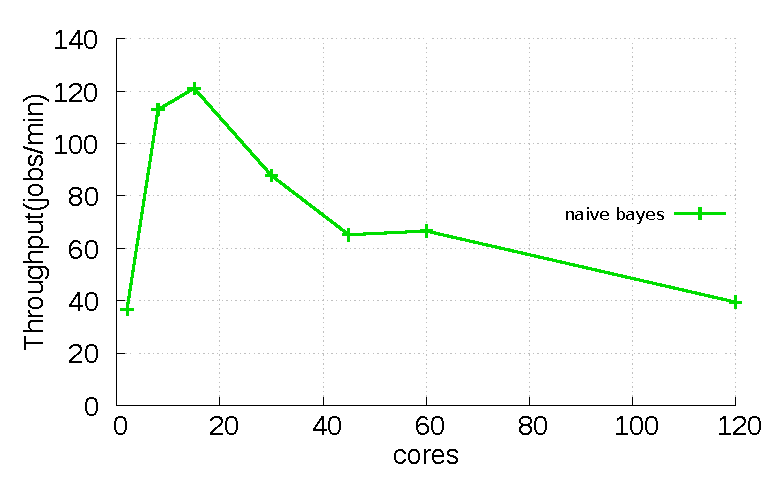
\includegraphics[width=2.2in]{graph/nb.eps}
        \caption{Naive Basian}
    \end{subfigure}%
    \begin{subfigure}[b]{0.33\textwidth}
        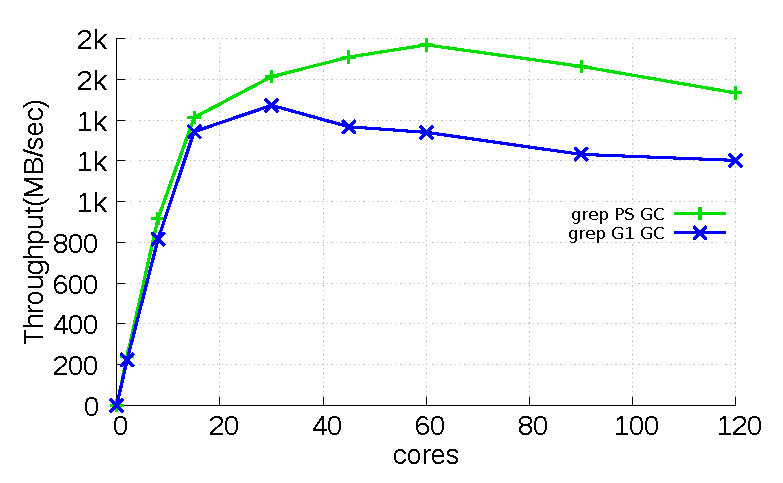
\includegraphics[width=2.2in]{graph/grep.eps}
        \caption{Grep}
    \end{subfigure}
        \begin{subfigure}[b]{0.33\textwidth}
        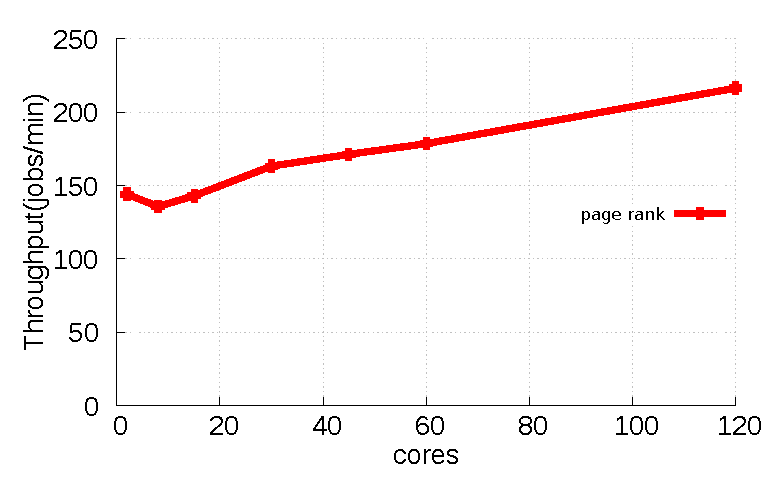
\includegraphics[width=2.2in]{graph/pagerank.eps}
        \caption{Pagerank}
    \end{subfigure}%
     \begin{subfigure}[b]{0.33\textwidth}
        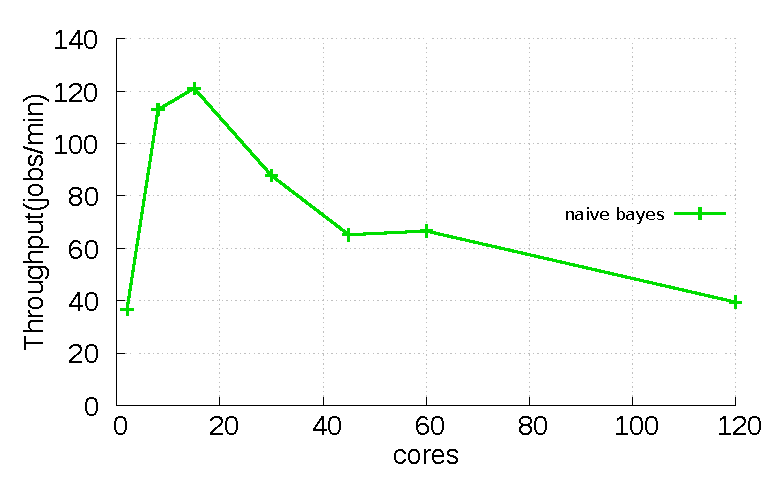
\includegraphics[width=2.2in]{graph/nb.eps}
        \caption{Naive Basian}
    \end{subfigure}%
    \begin{subfigure}[b]{0.33\textwidth}
        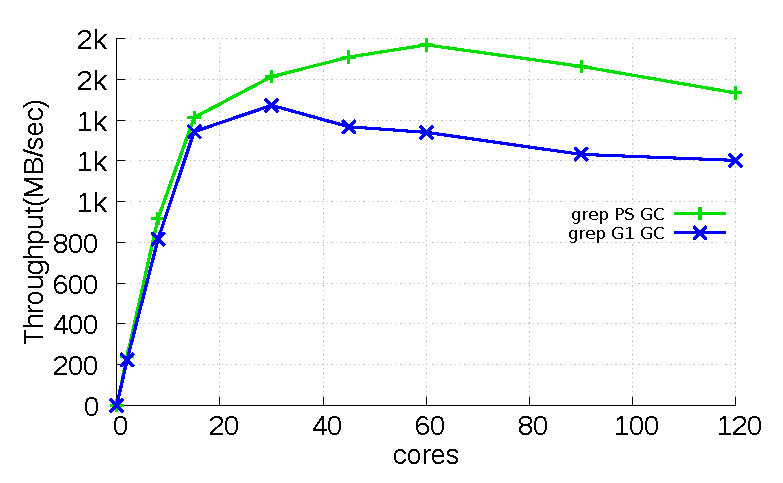
\includegraphics[width=2.2in]{graph/grep.eps}
        \caption{Grep}
    \end{subfigure}
    
        \centering
    \caption{CPU utilization on 120 core.}
    \label{fig:utilization}
\end{figure*}


%$$$$$$$$$$$$$$$$$$$$$$$$$$$$$$$$$$$$$$$$$$$$$$$$$$$$$$$$$$$$$$$$$$$$$$$$$$$$$$$$
%$$$$$$$$$$$$$$$$$$$$$$$$$$$$$$$$$$$$$$$$$$$$$$$$$$$$$$$$$$$$$$$$$$$$$$$$$$$$$$$$
%Scalability 결과에 대한 설명
%$$$$$$$$$$$$$$$$$$$$$$$$$$$$$$$$$$$$$$$$$$$$$$$$$$$$$$$$$$$$$$$$$$$$$$$$$$$$$$$$


\begin{figure*}[tb]
    \centering
    \begin{subfigure}[b]{0.25\textwidth}
        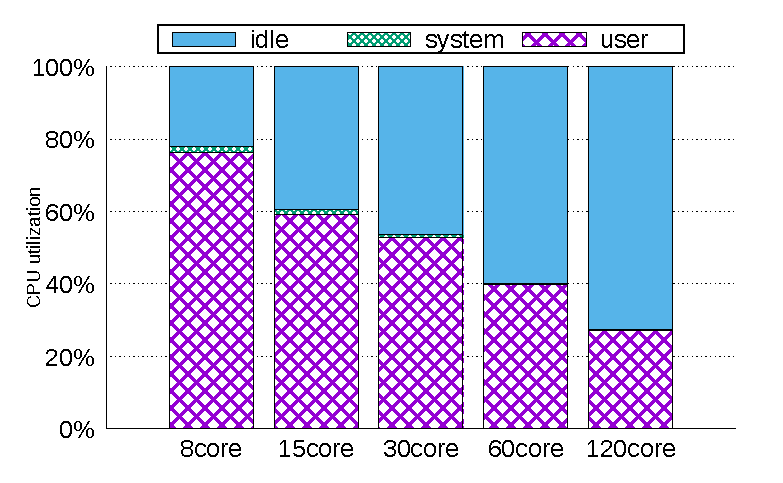
\includegraphics[width=1.8in]{graph/wc_cpuutils.eps}
        \caption{Word Count}
    \end{subfigure}%
    \begin{subfigure}[b]{0.25\textwidth}
        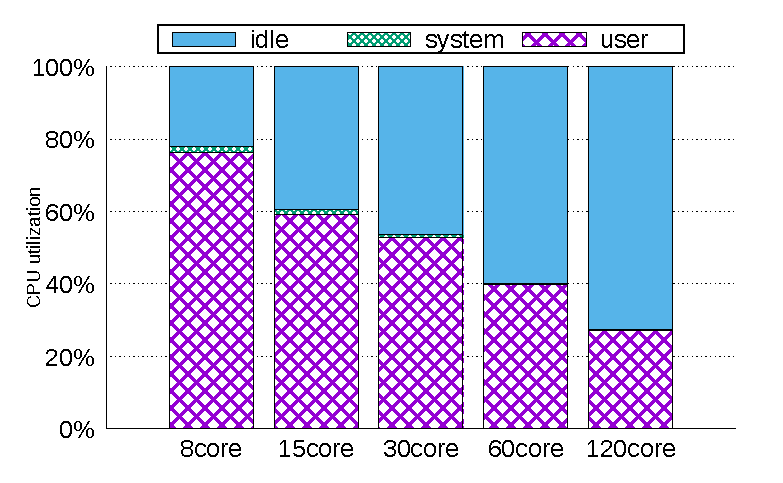
\includegraphics[width=1.8in]{graph/wc_cpuutils.eps}
        \caption{Naive Basian}
    \end{subfigure}%
    \begin{subfigure}[b]{0.25\textwidth}
        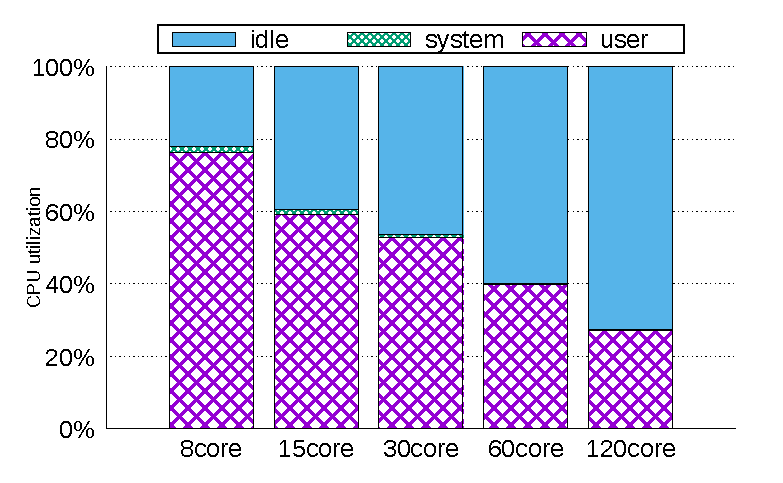
\includegraphics[width=1.8in]{graph/wc_cpuutils.eps}
        \caption{Grep}
    \end{subfigure}%
        \begin{subfigure}[b]{0.25\textwidth}
        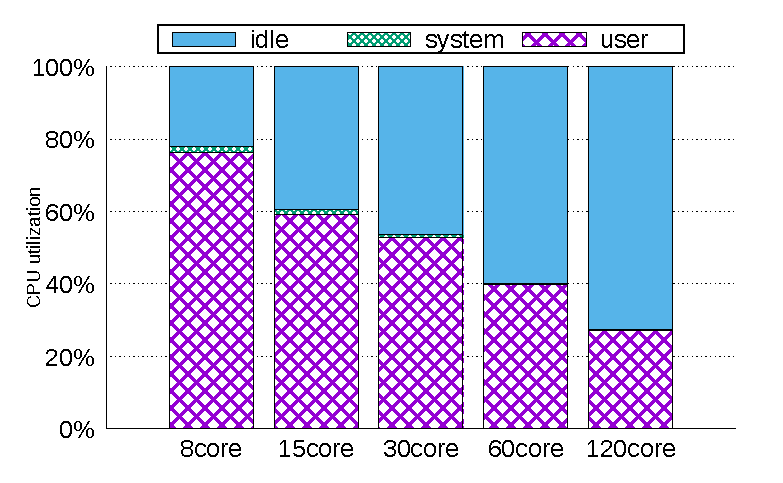
\includegraphics[width=1.8in]{graph/wc_cpuutils.eps}
        \caption{Pagerank}
    \end{subfigure}
        \centering
    \caption{CPU utilization on 120 core.}
    \label{fig:utilization}
\end{figure*}
Figure~\ref{fig:utilization}(a)) since it waits to acquire

\ifkor
벤치마크와 워크로드에 대한 BigData Benchmark를 사용하였다.
\else

\fi


%$$$$$$$$$$$$$$$$$$$$$$$$$$$$$$$$$$$$$$$$$$$$$$$$$$$$$$$$$$$$$$$$$$$$$$$$$$$$$$$$
%$$$$$$$$$$$$$$$$$$$$$$$$$$$$$$$$$$$$$$$$$$$$$$$$$$$$$$$$$$$$$$$$$$$$$$$$$$$$$$$$
%Lock에 대한 설명
%$$$$$$$$$$$$$$$$$$$$$$$$$$$$$$$$$$$$$$$$$$$$$$$$$$$$$$$$$$$$$$$$$$$$$$$$$$$$$$$$

\ifkor
벤치마크와 워크로드에 대한 BigData Benchmark를 사용하였다.
\else

\fi



%$$$$$$$$$$$$$$$$$$$$$$$$$$$$$$$$$$$$$$$$$$$$$$$$$$$$$$$$$$$$$$$$$$$$$$$$$$$$$$$$
%$$$$$$$$$$$$$$$$$$$$$$$$$$$$$$$$$$$$$$$$$$$$$$$$$$$$$$$$$$$$$$$$$$$$$$$$$$$$$$$$
%Perf에 대한 설명
%$$$$$$$$$$$$$$$$$$$$$$$$$$$$$$$$$$$$$$$$$$$$$$$$$$$$$$$$$$$$$$$$$$$$$$$$$$$$$$$$

\ifkor
벤치마크와 워크로드에 대한 BigData Benchmark를 사용하였다.
\else

\fi




